\chapter{Introduction}

\section{Flow in Magnetic Mirror Configuration}
Plasma flow in magnetic mirror configurations have been studied extensively in plasma physics due to its frequent precense in many areas such as the accretion flow\cite{jockers_stability_1968,aikawa_stability_1979} , and magnetic nozzle\cite{smolyakov_quasineutral_2021}. However, the stability of these configurations remains a debatable subject.



Despite these efforts, the stability of magnetic mirror configurations remains a topic of active research. New diagnostic techniques and advanced numerical simulations are being developed to improve our understanding of the underlying physics and guide the design of more stable magnetic nozzle.

\subsection{Magnetic Nozzle}
Magnetic nozzle is a convergent-divergent magnetic field that guides, expands and accelerates a plasma jet into vacuum for the purpose of space propulsion. \cite{andersen_continuous_1969,boswell_experimental_2004,williams_fusion_2003} The configuration is of the magnetic field in the magnetic nozzle plays a similar role to the walls of a Laval nozzle, see Fig. \ref{fig:magnetic-nozzle}. The plasma flow starts from subsonic at one end can be accelerated to supersonic at the exit. 

\begin{figure}[h]
	\centering
	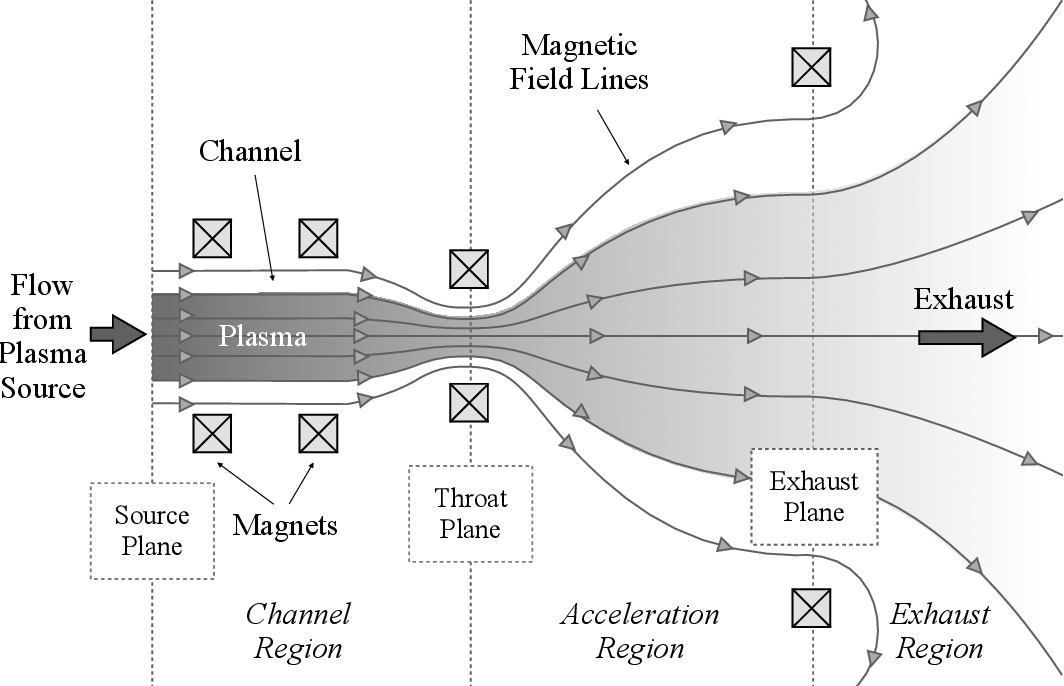
\includegraphics[width=0.7\linewidth]{img/introduction/magnetic_nozzle}
	\caption{Example of a magnetic nozzle configuration. In our models, we define the magnetic nozzle as the region downstream from the throat plane, which can be further divided into an acceleration region and exhaust region. The channel connects the plasma source (not shown) with the magnetic nozzle. \cite{little_performance_2015}}
	\label{fig:magnetic-nozzle}
\end{figure}


\subsection{Accretion Flow}
Accretion flow is similar to that in magnetic nozzle. The plasma flow is at rest at infinity and accelerated towards the steller object due to gravity. It is natural to compare the study of its instabilities to that of magnetic nozzle. However, the results are still debatable. \cite{keto_stability_2020,aikawa_stability_1979,stellingwerf_stability_1978}


\section{Goals of this Thesis}
The goals of this thesis is to first study the spectral method for solving the instability problem. When using the spectral method, it is necessary to understand different discretizations of the operators, such as finite difference, finite element and spectral element method.

Once the spectral method is introduced, we can use it to study the instability of plasma in magnetic nozzle. We can use different discretization techniques, and compare the results from different methods.

Finally, we need to take care of the filtering of the spectral pollution.


